\documentclass[border=6pt]{standalone}
\usepackage{tikz}
\usepackage{pgfplots}
\pgfplotsset{compat=1.18}
\usetikzlibrary{arrows.meta,positioning,shapes.geometric,fit,backgrounds,calc,decorations.pathreplacing,patterns,pgfplots.groupplots}
\tikzset{
  blk/.style={rectangle, rounded corners=2pt, draw=black!70, thick, fill=blue!6,
              minimum height=8mm, minimum width=20mm, align=center, font=\small},
  io/.style={rectangle, rounded corners=6pt, draw=black!70, thick, fill=green!8,
             minimum height=8mm, align=center, font=\small},
  proc/.style={rectangle, draw=black!70, thick, fill=orange!10, minimum height=8mm,
               align=center, font=\small},
  dec/.style={diamond, aspect=2, draw=black!70, thick, fill=yellow!15, align=center, font=\footnotesize},
  warnbox/.style={rectangle, rounded corners=2pt, draw=red!60!black, thick, fill=red!7,
                  minimum height=8mm, align=center, font=\small},
  oklbox/.style={rectangle, rounded corners=2pt, draw=green!45!black, thick, fill=green!8,
                 minimum height=8mm, align=center, font=\small},
  ar/.style={-{Latex[length=2mm]}, thick},
  arl/.style={-{Latex[length=2mm]}, thick, dashed, draw=black!55},
  lbl/.style={font=\footnotesize\itshape, text=black!60},
}
\definecolor{good}{RGB}{34,139,34}
\definecolor{bad}{RGB}{178,34,34}
\definecolor{warn}{RGB}{218,165,32}
\definecolor{pesblue}{RGB}{0,45,98}
\definecolor{complete}{RGB}{30,125,79}
\definecolor{partial}{RGB}{176,106,0}
\definecolor{blocked}{RGB}{166,43,43}
\begin{document}
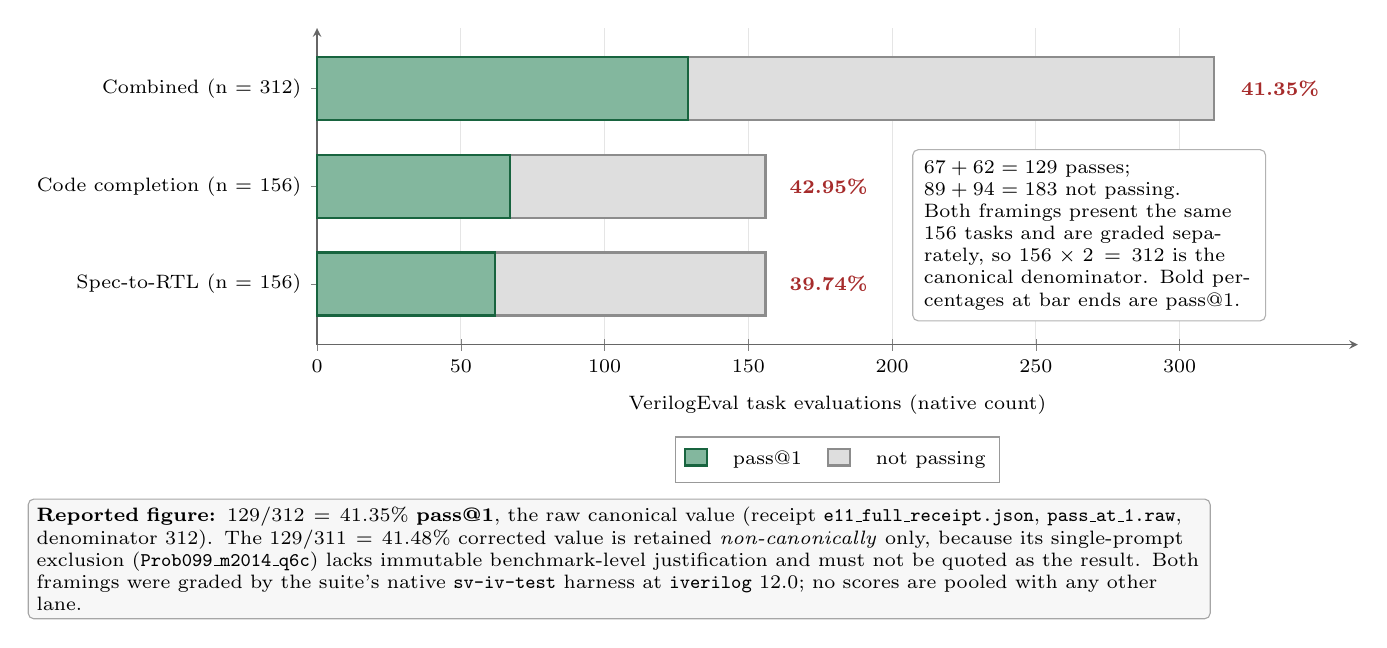
\begin{tikzpicture}
\begin{axis}[
  width=148mm, height=56mm,
  xbar stacked,
  bar width=8mm,
  xmin=0, xmax=362,
  ymin=-0.62, ymax=2.62,
  ytick={0,1,2},
  yticklabels={Spec-to-RTL (n = 156), Code completion (n = 156), Combined (n = 312)},
  yticklabel style={font=\scriptsize, align=right},
  xtick={0,50,100,150,200,250,300},
  xticklabel style={font=\scriptsize},
  xlabel={\scriptsize VerilogEval task evaluations (native count)},
  xlabel style={yshift=-1pt},
  xmajorgrids=true,
  grid style={draw=black!10},
  axis lines=left,
  axis line style={draw=black!60},
  clip=false,
  legend style={at={(0.5,-0.29)}, anchor=north, legend columns=2, font=\scriptsize,
                draw=black!40, fill=white, inner sep=3pt, column sep=7pt},
]
% ---- passing evaluations: the two framings, then their sum (real receipt counts) ----
\addplot[fill=complete!55, draw=complete!80!black, thick] coordinates {
  (129,2)
  (67,1)
  (62,0)
};
% ---- evaluations that did not pass: the remainder of each denominator ----
\addplot[fill=black!13, draw=black!45, thick] coordinates {
  (183,2)
  (89,1)
  (94,0)
};
\legend{pass@1, not passing}

% ---- counts printed on the bar segments (brief requirement) ----
% combined row (y = 2): green centre 129/2, grey centre 129 + 183/2
\node[font=\scriptsize, text=complete!35!black] at (axis cs:64.5,2)  {\textbf{129 / 312}};
\node[font=\scriptsize, text=black!70]         at (axis cs:220.5,2) {183};
% code-completion row (y = 1)
\node[font=\scriptsize, text=complete!35!black] at (axis cs:33.5,1)  {\textbf{67 / 156}};
\node[font=\scriptsize, text=black!70]         at (axis cs:111.5,1) {89};
% spec-to-RTL row (y = 0)
\node[font=\scriptsize, text=complete!35!black] at (axis cs:31,0)    {\textbf{62 / 156}};
\node[font=\scriptsize, text=black!70]         at (axis cs:109,0)   {94};

% ---- pass@1 rate at each bar end ----
\node[font=\scriptsize, text=blocked, anchor=west] at (axis cs:318,2) {\textbf{41.35\%}};
\node[font=\scriptsize, text=blocked, anchor=west] at (axis cs:161,1) {\textbf{42.95\%}};
\node[font=\scriptsize, text=blocked, anchor=west] at (axis cs:161,0) {\textbf{39.74\%}};

% ---- the decomposition arithmetic, in the free lower-right region ----
\node[draw=black!30, rounded corners=2pt, fill=white, font=\scriptsize,
      align=left, inner sep=4pt, anchor=west, text width=42mm]
  at (axis cs:207,0.5) {%
    $67 + 62 = 129$ passes;\\
    $89 + 94 = 183$ not passing.\\
    Both framings present the same 156 tasks and are graded separately, so
    $156 \times 2 = 312$ is the canonical denominator. Bold percentages at
    bar ends are pass@1.};
\end{axis}

% ---- provenance: canonical figure vs. the non-canonical sensitivity ----
\node[draw=black!35, fill=black!3, rounded corners=2pt, font=\scriptsize,
      align=left, inner sep=3pt, text width=148mm, anchor=north west]
  at ($(current bounding box.south west)+(0,-2mm)$)
  {\textbf{Reported figure: $129/312 = 41.35\%$ pass@1}, the raw canonical value
   (receipt \texttt{e11\_full\_receipt.json}, \texttt{pass\_at\_1.raw}, denominator 312).
   The $129/311 = 41.48\%$ corrected value is retained \emph{non-canonically} only, because its
   single-prompt exclusion (\texttt{Prob099\_m2014\_q6c}) lacks immutable benchmark-level
   justification and must not be quoted as the result. Both framings were graded by the suite's
   native \texttt{sv-iv-test} harness at \texttt{iverilog} 12.0; no scores are pooled with any
   other lane.};

\end{tikzpicture}
\end{document}
